\documentclass{report}
\usepackage{ctex}
\usepackage{graphicx}
\usepackage{amsmath}
\usepackage{indentfirst}
\usepackage{titlesec}
\usepackage{setspace}
\usepackage{subfigure}
\usepackage{caption}
\usepackage{float}
\usepackage{booktabs}
\title{\songti \zihao{2}\bfseries 氢氘原子光谱}
\titleformat*{\section}{\songti\zihao{4}\bfseries}
\titleformat*{\subsection}{\songti\zihao{5}\bfseries}
\renewcommand\thesection{\arabic{section}}
\author{王启骅 PB20020580}
\begin{document}
	\maketitle
	\section{实验目的}
学习光谱仪等仪器的使用。通过测量氢氘原子光谱3、4、5、6级谱线的波长,计算氢氘谱线的里德伯常数、氢氘核质量比和质子电子质量比。
	\section{实验原理}

氢原子光谱在可见光区的谱线系是巴耳末系,其代表线为$ H_{\alpha}\quad H_{\beta}\quad H_{\gamma}\quad H_{\delta} $,这些谱线的间隔和强度都向着短波方向递减,并满足下列规律:
	\begin{equation}
		\lambda=364.56\dfrac{n^2}{n^2-4}
	\end{equation}


 若用波数$ \tilde{\nu}=1/\lambda $表示谱线,则式(1)可写为:
 	\begin{equation}
 	\nu=R_H(\frac{1}{2^2}-\frac{1}{n^2})
 \end{equation}


根据波尔理论和量子力学对氢原子和氘原子里德伯常量的分析有:
 	\begin{equation}
	R_H=\dfrac{R_{\infty}}{1+m_e/M_H}
\end{equation}
 	\begin{equation}
	R_D=\dfrac{R_{\infty}}{1+m_e/M_D}
\end{equation}
 	\begin{equation}
	R_{\infty}=\dfrac{2\pi^2me^4}{(4\pi \epsilon_0)^2ch^3}
\end{equation}


$ M_h \quad M_D $分别表示氢与氘原子核的质量。由(3)、(4)解得:
 	\begin{equation}
\frac{M_D}{M_h}=\dfrac{R_D/R_H}{1-(R_D/R_H-1)M_H/m_e}
\end{equation}


根据氢与氘的巴耳末系公式形式相同:
 	\begin{equation}
	\frac{1}{\lambda_H}=R_H(\frac{1}{2^2}-\frac{1}{n^2})
\end{equation}
 	\begin{equation}
	\frac{1}{\lambda_D}=R_D(\frac{1}{2^2}-\frac{1}{n^2})
\end{equation}


可得:
 	\begin{equation}
	\frac{M_D}{M_h}=\frac{m}{M_H}\cdot\dfrac{\lambda_H}{\lambda_D-\lambda_H+\lambda_D m/M_H}
\end{equation}


这样实验中只要测得各谱线的$ \lambda_H $或$ \lambda_D $ ,并辨认出与各谱线对应的 n,即可算出$ R_H $与$ R_D $
以及氢氘质量比。


同时,我们可以根据测量的波长计算氢氘谱峰波长差 :
 	\begin{equation}
\Delta \lambda=(\frac{1}{R_H}-\frac{1}{R_D})/(\frac{1}{2^2}-\frac{1}{n^2})\approx\dfrac{\frac{M+m}{M}-\frac{2M+m}{2M}}{1/\lambda}=\frac{m}{2M}\lambda
\end{equation}


即:
 	\begin{equation}
\frac{M}{m}\approx\frac{\lambda}{2\Delta\lambda}
\end{equation}
	\section{实验仪器}
控制电源、汞灯、氢氘灯、光谱仪、光电倍增管、计算机。
	\section{数据处理}
	\subsection{实验数据表格}
\begin{table}[!h]
		\centering
	\captionsetup{font={small},labelfont=bf}
	\caption{\heiti\zihao{-5}汞灯谱线波长}
	\begin{tabular}{|c|c|c|c|c|c|}
		
		\hline
		汞灯谱线序号&1&2&3&4&5\\
				\hline
		波长/nm&364.90&365.38&366.22&404.67&407.77\\
				\hline
		汞灯谱线序号&6&7&8&9&\\
				\hline
		波长/nm&435.73&546.61&577.67&579.64&\\
				\hline
	\end{tabular}
\end{table}
	\begin{table}[!h]
		\centering
		\captionsetup{font={small},labelfont=bf}
		\caption{\heiti\zihao{-5}氢氘灯光谱波长}
		\begin{tabular}{|c|c|c|c|c|}
			
			\hline
			能级n&6&5&4&3\\
			\hline
			波长$ \lambda_H $/nm&410.01&433.96&486.38&657.94\\
			\hline
		
			波长$ \lambda_D $/nm&409.92&433.88&486.25&657.77\\
			\hline
		\end{tabular}
	\end{table}
\subsection{汞灯标准谱线和测量谱线拟合方程和拟合图}
 \begin{figure}
	\centering
	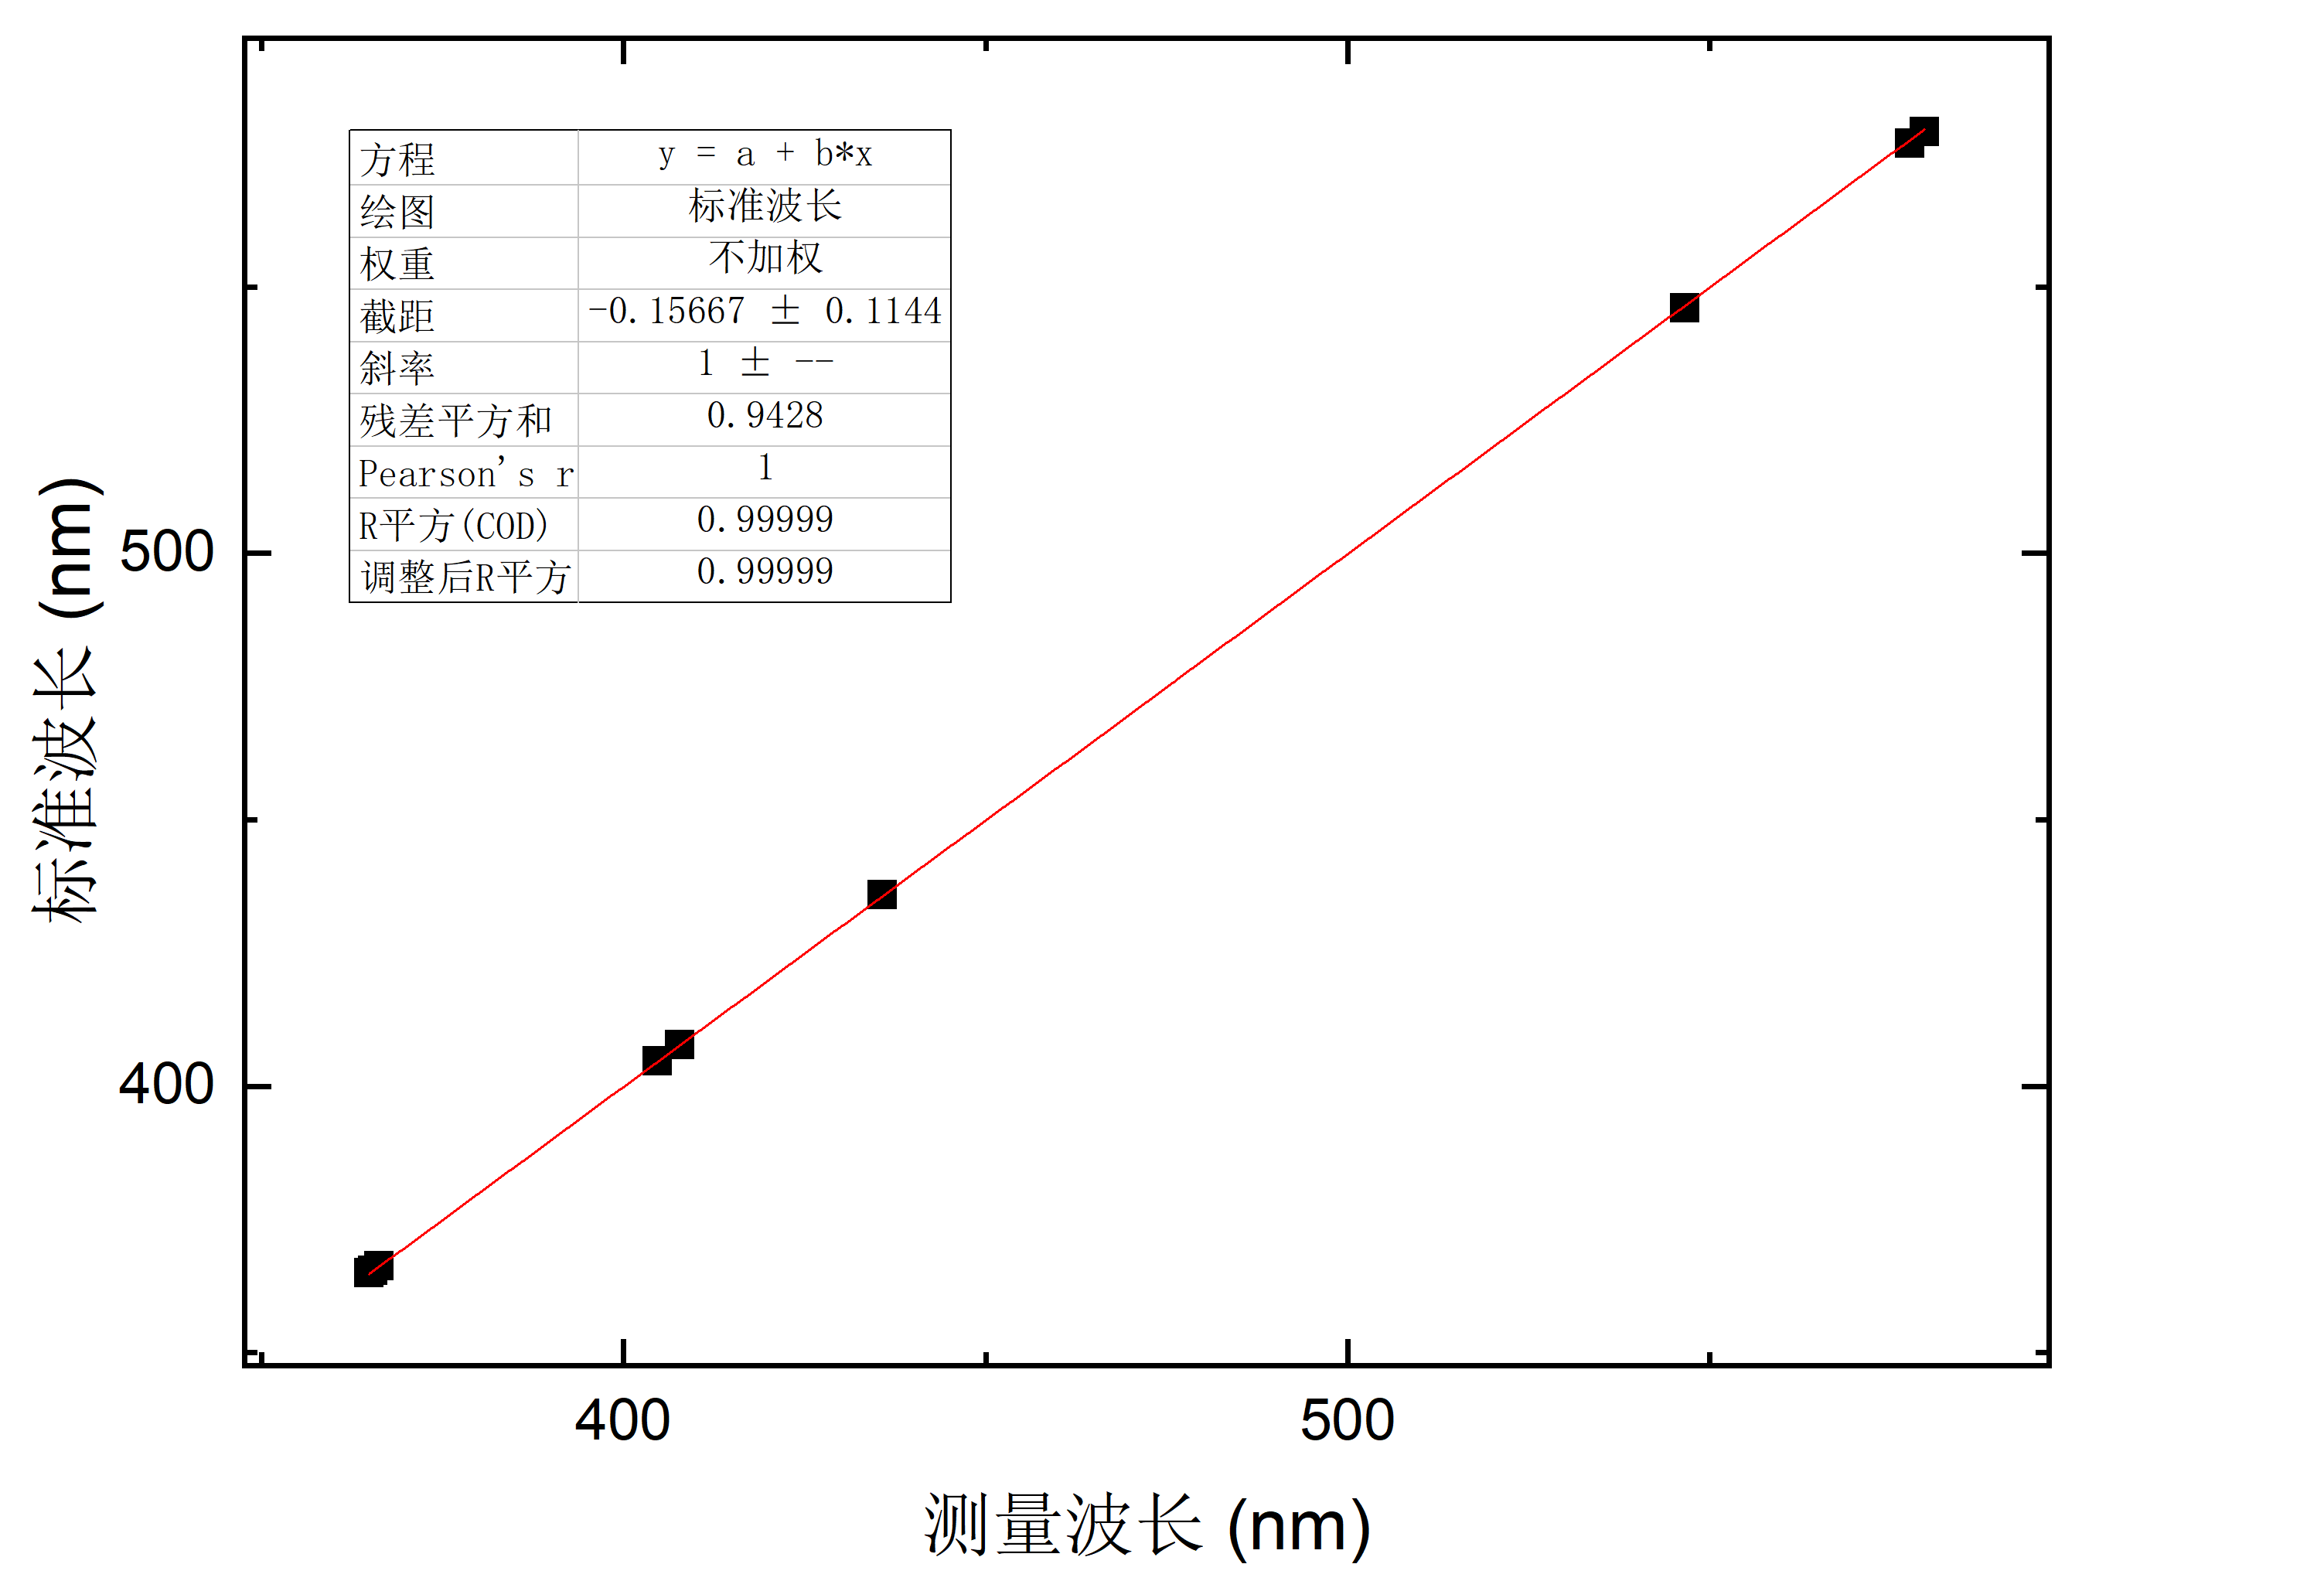
\includegraphics[scale=0.12]{汞灯拟合}
	\captionsetup{font={small},labelfont=bf}
	\caption{\heiti\zihao{-5}汞灯校准拟合图}
	
\end{figure}
根据拟合结果得到转换关系方程:
$ \lambda_{stan}=\lambda_{meas}-0.15667 $
\subsection{氢氘谱线校准后数据}
	\begin{table}[!h]
	\centering
	\captionsetup{font={small},labelfont=bf}
	\caption{\heiti\zihao{-5}校准后氢氘灯光谱波长}
	\begin{tabular}{|c|c|c|c|c|}
	
	\hline
	能级n&6&5&4&3\\
	\hline
	波长$ \lambda_H $/nm&409.85&433.80&486.22&657.78\\
	\hline

	波长$ \lambda_D $/nm&409.76&433.72&486.09&657.61\\
	\hline


\end{tabular}
\end{table}
\subsection{实验结果计算}
对$ \dfrac{1}{\lambda} $关于$ \dfrac{1}{2^2}-\dfrac{1}{n^2} $ 线性拟合得到斜率即为里德伯常量数值。由图2、3得到
\begin{equation}
	R_H=(1.0972\pm0.0006)\times10^7 m^{-1}  \nonumber
\end{equation}
\begin{equation}
	R_D=(1.0975\pm0.0006)\times10^7 m^{-1}  \nonumber
\end{equation}

 \begin{figure}
	\centering
	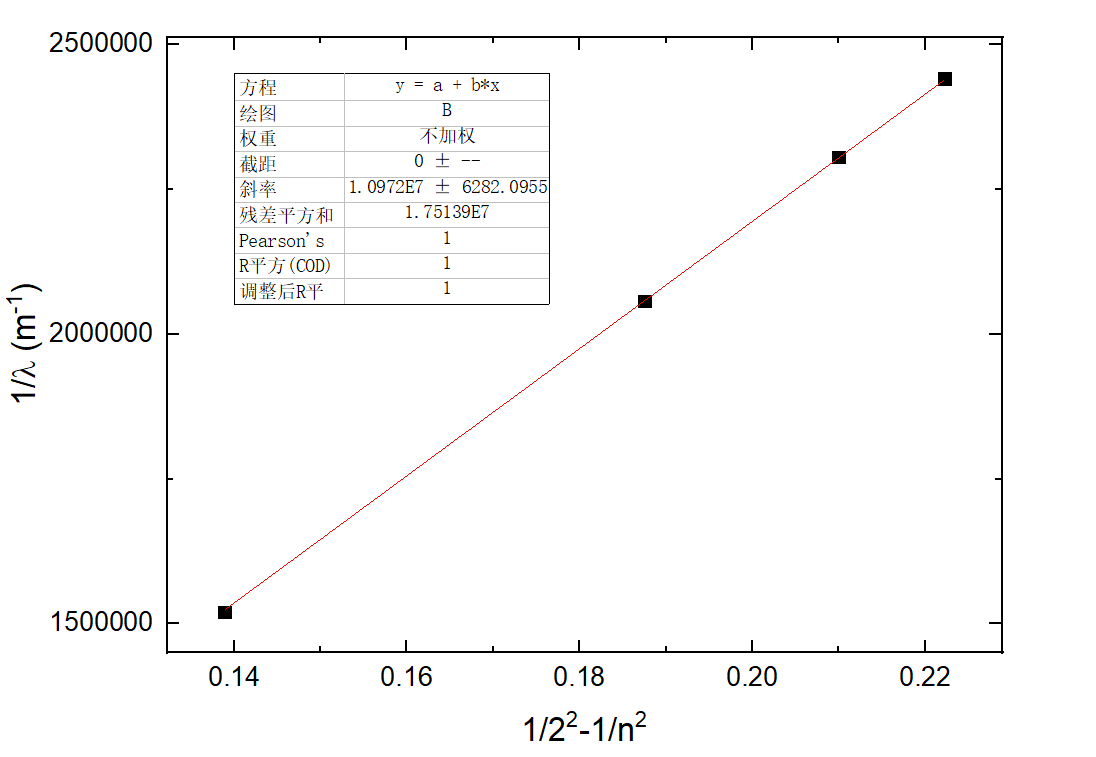
\includegraphics[scale=0.5]{R_H拟合}
	\captionsetup{font={small},labelfont=bf}
	\caption{\heiti\zihao{-5}氢原子谱线拟合图}
	
\end{figure}
 \begin{figure}
	\centering
	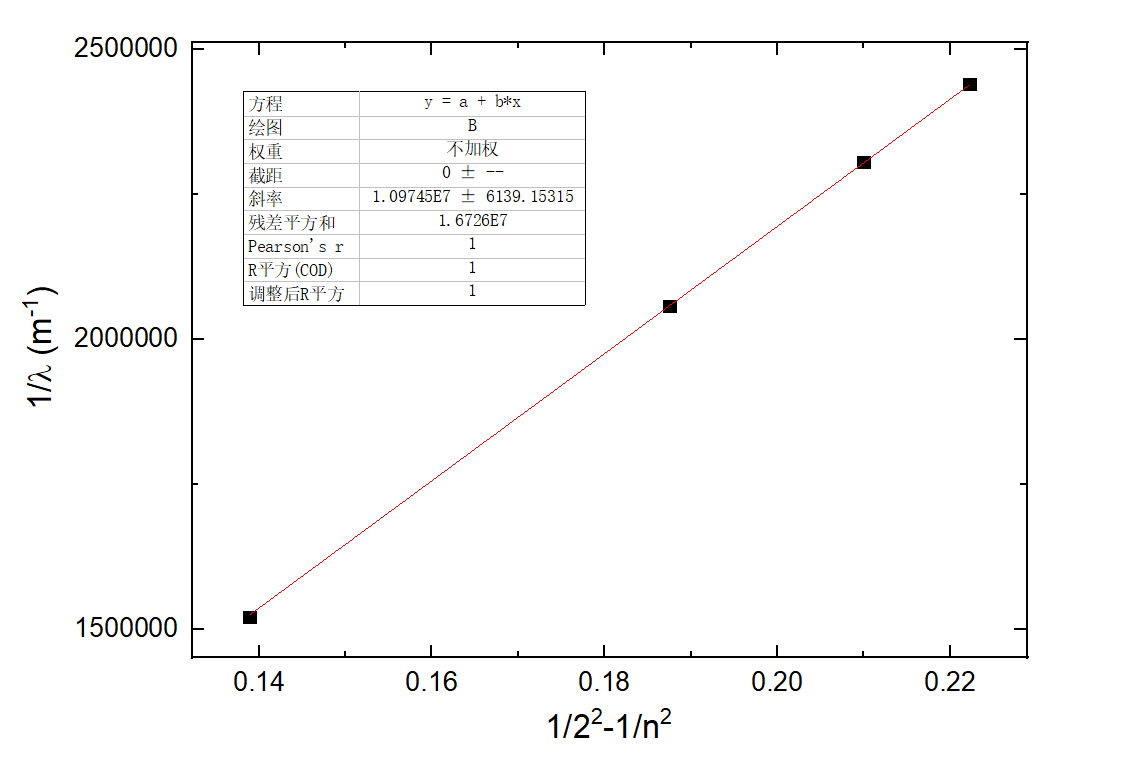
\includegraphics[scale=0.5]{R_D拟合}
	\captionsetup{font={small},labelfont=bf}
	\caption{\heiti\zihao{-5}氘原子谱线拟合图}
	
\end{figure}


带入公式(6)可得:
\begin{equation}
	\frac{M_D}{M_H}=\dfrac{1.0975/1.0972}{1-(1.0975/1.0972-1)\cdot1836.1527}=2.0088\nonumber
\end{equation}


对$\lambda$根据$ 2\Delta\lambda $线性拟合可以得到拟合直线斜率即为质子与电子质量比
 \begin{figure}[!h]
	\centering
	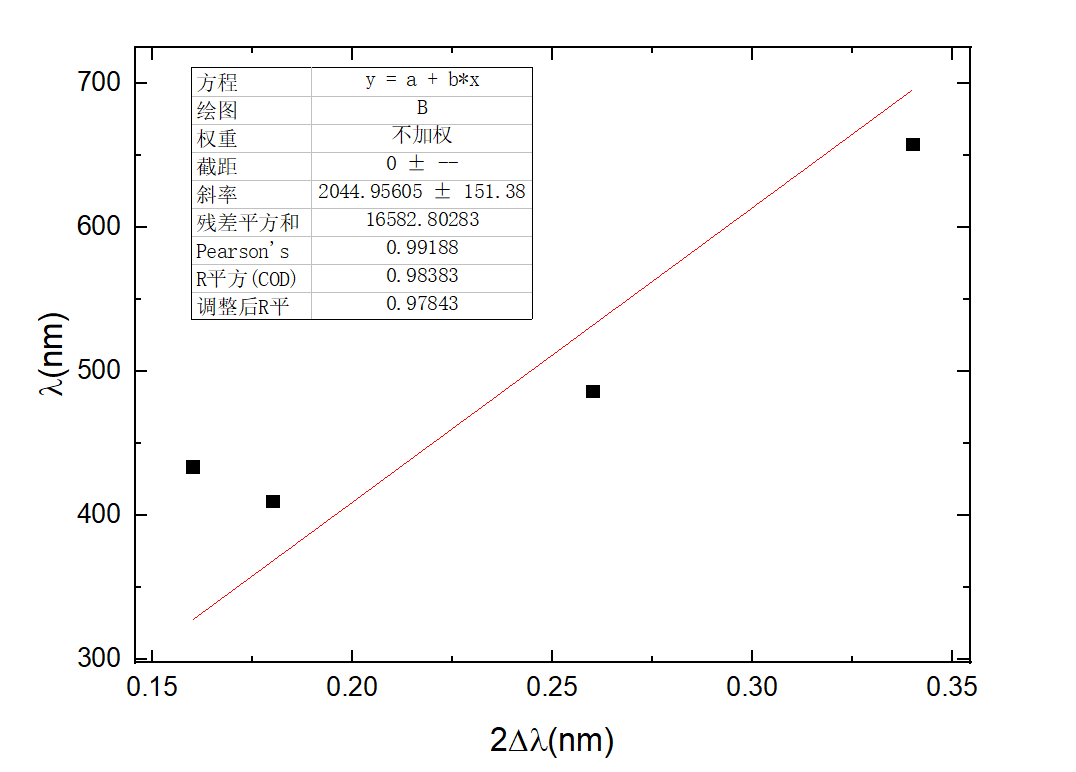
\includegraphics[scale=0.5]{质子电子比}
	\captionsetup{font={small},labelfont=bf}
	\caption{\heiti\zihao{-5}$ \lambda $关于$ 2\Delta\lambda $线性拟合图}
	
\end{figure}


根据图(4)得到:
\begin{equation}
	\frac{M_H}{m_e}=2045.0\pm151.4 \nonumber
\end{equation}
	\section{实验结果误差分析}
\begin{equation}
 \dfrac{U_{\frac{R_D}{R_H}}}{\frac{R_D}{R_H}}=\sqrt{(\dfrac{U_{R_H}}{R_H})^2+(\dfrac{U_{R_D}}{R_D})^2}=\sqrt{(\dfrac{0.0006}{1.0972})^2+(\dfrac{0.0006}{1.0975})^2}=8\times10^{-4} \nonumber
\end{equation}
, P=0.95

\begin{equation}
	\dfrac{U_{\frac{M_D}{M_H}}}{\frac{M_D}{M_H}}=\sqrt{(\dfrac{U_{\frac{R_D}{R_H}}}{\frac{R_D}{R_H}})^2+(\dfrac{M_H/m_eU_{\frac{R_D}{R_H}}}{M_H/m_e\frac{R_D}{R_H}})^2}=\sqrt{(8\times10^4)^2+(8\times10^4)^2}=1.1\times10^{-3} \nonumber
\end{equation}  
 , P=0.95
 
 
 则在P=0.95下,实验结果为:
 \begin{equation}
 	R_H=(1.0972\pm0.0006)\times10^7 m^{-1}  \nonumber
 \end{equation}
 \begin{equation}
 	R_D=(1.0975\pm0.0006)\times10^7 m^{-1}  \nonumber
 \end{equation}
\begin{equation}
	\frac{M_D}{M_H}=\dfrac{1.0975/1.0972}{1-(1.0975/1.0972-1)\cdot1836.1527}=2.0088\pm0.0022\nonumber
\end{equation}
\begin{equation}
	\frac{M_H}{m_e}=(2.05\pm0.15)\times10^3\nonumber
\end{equation}
	\section{思考题和实验总结}
\subsection{思考题}
1.由介质中波长公式:
\begin{equation}
	\lambda'=\lambda/n \nonumber
\end{equation}
得到修正公式:
\begin{equation}
		\frac{1}{n\lambda'}=R_H(\frac{1}{2^2}-\frac{1}{n^2}) \nonumber
\end{equation}
得到修正后$ R_H=1.0969\times10^7m^{-1} $ , $ R_D=1.0972\times10^7m^{-1} $\\
与公认值$ 1.0974\times10^7m^{-1} $分别相差$ 0.046\% $ , $ 0.020\% $


2.由于光谱仪本身测量存在一定误差,相较于零点有一定的偏移,通过测量汞灯的光谱并与标准谱线进行对比与线性拟合,可以得到直线的截距即为光谱仪零点的偏移量。在测量数据后需要加上零点偏移的修正项,以减少误差。


方案:选取一系列单色性较好的不同波长的激光器,且需要各个激光器的波长位于氢原子光谱附近。利用光谱仪测量各个激光器的波长后根据标准波长进行线性拟合,并求出拟合直线截距,作为零点的偏移量。


3.	要求需要提高仪器的分辨率。氢原子已经是原子序数最低的原子,随着原子序数的提高,位移效应越小,同位素发射的光波长越接近,难以测量出不同核素的光谱。因此需要提高仪器分辨率以区分不同核素的相同能级的谱线波长。

\subsection{实验总结}
通过本实验学习了光谱仪等仪器的使用,测量了氢氘原子光谱并计算得到了非近似情况下的里德伯常量数值、氢氘原子核质量比,和质子电子质量比。同时,实验结果与真是值存在一定偏差,主要原因为氢氘灯较弱,且光谱仪精度不足,难以探测出精确的波长差。
\end{document}